\section{Infidelity}\label{section:infidelity}

Infidelity \cite{yeh2019fidelity} comes from the idea of fidelity, which could be defined as the amount of how many features with high attributions belong to a priori subset of features that are relevant to the prediction. This definition assumes that we have such a subset of relevant features, and that is not a valid assumption in most situations. In another paper \cite{ancona2017towards}, Ancona et al. are trying to come up with a quantitative measure for the XAI methods, which has no human bias. The idea is to relate the new measure to the correlation between the importance of features and the change in models' prediction. This can be achieved by perturbing the input and calculating the correlation between the perturbation of features with the predicted score.

\begin{definition}[Infidelity]\label{def:infidelity}
    For a given model $F$, attribution method $\Phi$, input $x$, and significant perturbation around input $I$, \textit{infidelity} for an attribution method is defined as:
    
    \begin{equation}
        \operatorname{INFD}(\Phi, \mathbf{F}, \mathbf{x})=\mathbb{E}_{\mathbf{I} \sim \mu_{\mathrm{I}}}\left[\left(\mathbf{I}^{T} \Phi(\mathbf{F}, \mathbf{x})-(\mathbf{F}(\mathbf{x})-\mathbf{F}(\mathbf{x}-\mathbf{I}))\right)^{2}\right]
        \label{eq:infidelity}
    \end{equation}

\end{definition}

Infidelity measure (eq. \ref{eq:infidelity}) consists of two major part which expected difference is a measure of infidelity. The first part ($\mathbf{I}^{T} \Phi(\mathbf{F}, \mathbf{x})$) is a dot product between the perturbation and the attribution generated by the XAI method. Attribution used for the calculation is the attribution for the image without perturbation. This method does not rely on the attribution of the perturbed image anywhere. The second part $(\mathbf{F}(\mathbf{x})-\mathbf{F}(\mathbf{x}-\mathbf{I}))^{2}$ is a squared difference between the score of the original image and the perturbed image. The perturbation is usually drawn from the Gaussian distribution with the $\mu = 0$, and the $\sigma$ is the parameter.

\begin{wrapfigure}{L}{0.40\textwidth}
  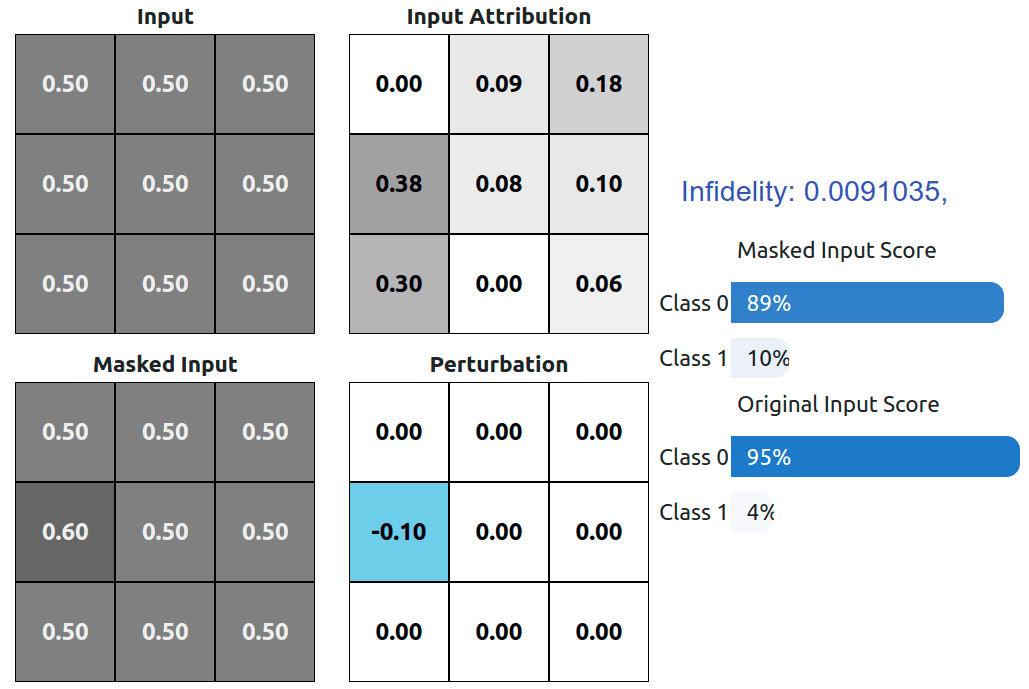
\includegraphics[width=0.40\textwidth]{methods/images/infidelity-small.png}
  \caption{Small perturbation of the feature value with the high initial attribution results in a small infidelity measure.}\label{fig:infidelity-small}
  \smallskip\par
  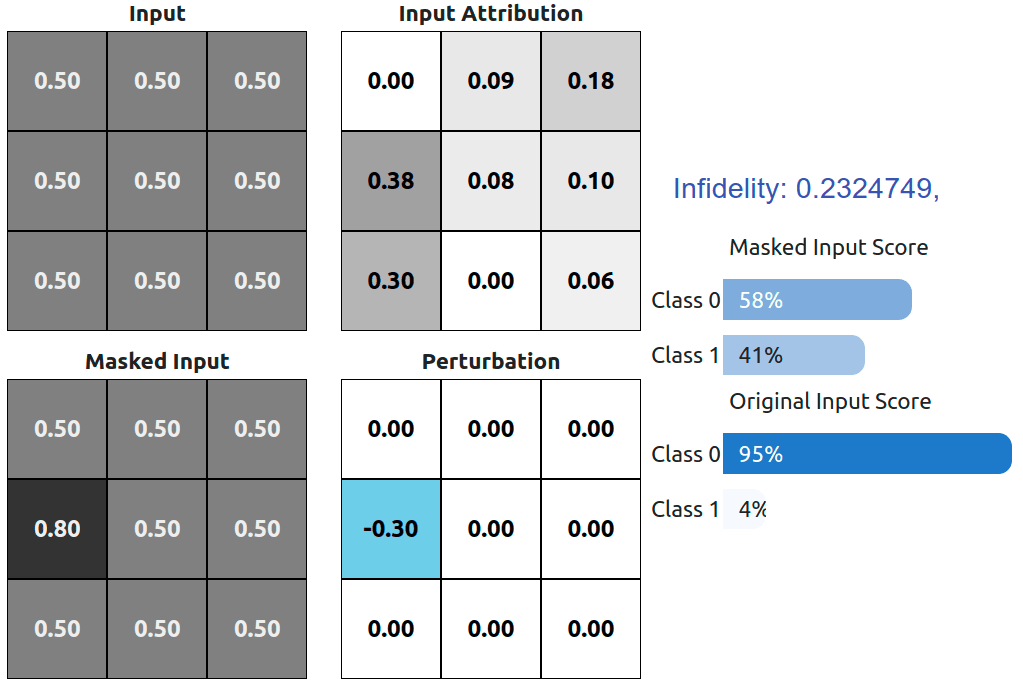
\includegraphics[width=0.40\textwidth]{methods/images/infidelity-large.png}
  \caption{High perturbation of the feature value with the high initial attribution results in a large infidelity measure.}\label{fig:infidelity-large}
\end{wrapfigure}

\vspace{\baselineskip}

To explain the intuition behind the infidelity measure as mentioned in section \ref{section:sensitivity}. This time the perturbation is done on the feature with high initial attribution of $0.38$. The first part of the equation is a dot product between transposed \textit{Perturbation} matrix and the \textit{Input Attribution} matrix. The second part is a difference between the \textit{Original Input Score} of class $0$ and the \textit{Masked Input Score} of class $0$.

\vspace{\baselineskip}

As shown in Figure \ref{fig:infidelity-small}, changing the feature with high attribution by a small amount ($-0.1$) resulted in a relatively small infidelity score of $0.0091$. This value is primarily due to a small change in the class prediction between input and the masked input. The next example (Fig. \ref{fig:infidelity-large}) shows a significantly larger value of infidelity. This time the change in score is greater in relation to change in the input features (score for class $0$ dropped by $0.37$ for $0.3$ change in the value of the feature). 

\vspace{\baselineskip}

These two examples show how infidelity behaves and what it tries to measure. If the initial attribution of the feature is correct, then the infidelity values should be close to zero. If the correlation between attribution value and the change in models' prediction varies, then the infidelity values should be higher. By definition, the measure checks if the fidelity of the attributions relates to what the model predicts.